\documentclass[12pt, a4paper]{article} 
\usepackage{fontspec} % Font selection for XeLaTeX; see fontspec.pdf. 

\usepackage{xeCJK}	% 中文使用 XeCJK,利用 \setCJKmainfont 定義中文內文、粗體與斜體的字型
%\usepackage[BoldFont, SlantFont]{xeCJK}
% 中文使用 XeCJK,並模擬粗體與斜體(\textbf{ } \textit{ })

\defaultfontfeatures{Mapping=tex-text} 
% to support TeX conventions like ``---''
\usepackage{xunicode} 
% Unicode support for LaTeX character names(accents, European chars, etc)
\usepackage{xltxtra} 				
% Extra customizations for XeLaTeX
\usepackage{amsmath, amssymb}
\usepackage{enumerate}
\usepackage{graphicx, subfig, float, wrapfig} 
% support the \includegraphics command and options
\usepackage[outercaption]{sidecap} 
%[options]=[outercaption], [innercaption], [leftcaption], [rightcaption]
\usepackage{array, booktabs}
\usepackage{color, xcolor}
% 跨頁的超長表格;lscape是旋轉此類表格的
\usepackage{longtable, lscape}              
% 巨集,使表格加註解更容易(手冊p169)
\usepackage{threeparttable}      
% 讓表格編起來更美的套件(手冊p166),編輯跨列標題重覆的表格(手冊p182)           
\usepackage{multirow, booktabs}             
\usepackage{colortbl}     
% 直接將 latex 碼轉換成顯示文字   
\usepackage{listings}						
% 新段落前加一空行,不使用縮排

\usepackage[parfill]{parskip} 				
% 新段落前加一空行,不使用縮排

\usepackage{geometry} 
% See geometry.pdf to learn the layout options. There are lots.
%\usepackage[left=3in,right=3in,top=2in,bottom=2in]{geometry} 

\usepackage{url}

%.....表格標題註解之巨集套件.....%
% for Reference
\usepackage{natbib}			
% for Indexing				
\usepackage{makeidx}		
% Activate to begin paragraphs with an empty line rather than an indent

%章節設定
\usepackage{titlesec, titletoc,CJKnumb}		


%-----------------------------------------------------------------
%  中英文內文字型設定
%\setCJKmainfont							% 設定中文內文字型
%	[
		%BoldFont=Microsoft YaHei	    %定義粗體的字型(Win)
%		BoldFont=蘋果儷中黑	    		%定義粗體的字型(Mac)
%	]
%	{新細明體}						% 設定中文內文字型(Win)
%	{宋體-繁}							% 設定中文內文字型(Mac)	
%\setmainfont{Times New Roman}		% 設定英文內文字型
%\setsansfont{Arial}					% 無襯字字型 used with {\sffamily ...}
%\setsansfont[Scale=MatchLowercase,Mapping=tex-text]{Gill Sans}
%\setmonofont{Courier New}			% 等寬字型 used with {\ttfamily ...}
%\setmonofont[Scale=MatchLowercase]{Andale Mono}


% 英文字型
%\newfontfamily{\E}{Calibri}				
%\newfontfamily{\A}{Arial}
%\newfontfamily{\C}[Scale=0.9]{Arial}
%\newfontfamily{\R}{Times New Roman}
%\newfontfamily{\TT}[Scale=0.8]{Times New Roman}

% 中文字型
%\newCJKfontfamily{\MB}{微軟正黑體}				% 等寬及無襯線字體 Win
%\newCJKfontfamily{\SM}[Scale=0.8]{新細明體}	% 縮小版(Win)
%\newCJKfontfamily{\K}{標楷體}                	% Windows下的標楷體
%\newCJKfontfamily{\BB}{Microsoft YaHei}		% 粗體 Win
%\newCJKfontfamily{\CF}{cwTeX Q Fangsong Medium}	% CwTex 仿宋體
%\newCJKfontfamily{\CB}{cwTeX Q Hei Bold}			% CwTex 粗黑體
%\newCJKfontfamily{\CK}{cwTeX Q Kai Medium}   	% CwTex 楷體
%\newCJKfontfamily{\CM}{cwTeX Q Ming Medium}		% CwTex 明體
%\newCJKfontfamily{\CR}{cwTeX Q Yuan Medium}		% CwTex 圓體
%----------------------------------------------------------
%  中英文內文字型設定
\setCJKmainfont							% 設定中文內文字型
	[
%		BoldFont=Microsoft YaHei	    % 定義粗體的字型(Win)
		BoldFont=黑體-繁	    		    % 定義粗體的字型(Mac)
	]
%	{新細明體}						    % 設定中文內文字型(Win)
	{宋體-繁}							% 設定中文內文字型(Mac)	
\setmainfont{Times New Roman}		    % 設定英文內文字型
\setsansfont{Arial}					    % 無襯字字型 used with {\sffamily ...}
%\setsansfont[Scale=MatchLowercase,Mapping=tex-text]{Gill Sans}
\setmonofont{Courier New}			    % 等寬字型 used with {\ttfamily ...}
%\setmonofont[Scale=MatchLowercase]{Andale Mono}
% 其他字型(隨使用的電腦安裝的字型不同,用註解的方式調整(打開或關閉))
% 英文字型
\newfontfamily{\A}{Arial}
\newfontfamily{\C}{Cochin}				
\newfontfamily{\SA}[Scale=0.9]{Arial}
\newfontfamily{\R}{Times New Roman}
\newfontfamily{\ST}[Scale=0.8]{Times New Roman}
% 中文字型
%\newCJKfontfamily{\MB}{微軟正黑體}				    % 等寬及無襯線字體 Win
\newCJKfontfamily{\MB}{黑體-繁}				        % 等寬及無襯線字體 Mac
%\newCJKfontfamily{\SM}[Scale=0.8]{新細明體}	        % 縮小版(Win)
\newCJKfontfamily{\SM}[Scale=0.8]{宋體-繁}	        % 縮小版(Mac)
%\newCJKfontfamily{\K}{標楷體}                	    % Windows下的標楷體
\newCJKfontfamily{\K}{黑體-繁}               	    % Mac下的標楷體
%\newCJKfontfamily{\BB}{Microsoft YaHei}		    % 粗體 Win
\newCJKfontfamily{\BB}{宋體-繁}		                % 粗體 Mac
% 以下為自行安裝的字型:CwTex 組合
%\newCJKfontfamily{\CF}{cwTeX Q Fangsong Medium}	% CwTex 仿宋體
%\newCJKfontfamily{\CB}{cwTeX Q Hei Bold}			% CwTex 粗黑體
%\newCJKfontfamily{\CK}{cwTeX Q Kai Medium}   	    % CwTex 楷體
%\newCJKfontfamily{\CM}{cwTeX Q Ming Medium}		% CwTex 明體
%\newCJKfontfamily{\CR}{cwTeX Q Yuan Medium}		% CwTex 圓體
%-------------------------------------------------------------
\XeTeXlinebreaklocale "zh"             		
%這兩行一定要加,中文才能自動換行
\XeTeXlinebreakskip = 0pt plus 1pt     		
%這兩行一定要加,中文才能自動換行
%-----------------------------------------------------------------------------------------------------------------------


\newcommand{\cw}{\texttt{cw}\kern-.6pt\TeX}	% 這是 cwTex 的 logo 文字
\newcommand{\imgdir}{/Users/guoyixuan/Documents/NTPU_STAT/images/}				% 設定圖檔的目錄位置
\renewcommand{\tablename}{表}					% 改變表格標號文字為中文的「表」(預設為 Table)
\renewcommand{\figurename}{圖}				% 改變圖片標號文字為中文的「圖」(預設為 Figure)
\usepackage{booktabs}


% 設定顏色 see color Table: http://latexcolor.com
\usepackage{color}
\definecolor{slight}{gray}{0.9}				
\definecolor{airforceblue}{rgb}{0.36, 0.54, 0.66} 
\definecolor{arylideyellow}{rgb}{0.91, 0.84, 0.42}
\definecolor{babyblue}{rgb}{0.54, 0.81, 0.94}
\definecolor{cadmiumred}{rgb}{0.89, 0.0, 0.13}
\definecolor{coolblack}{rgb}{0.0, 0.18, 0.39}
\definecolor{beaublue}{rgb}{0.74, 0.83, 0.9}
\definecolor{beige}{rgb}{0.96, 0.96, 0.86}
\definecolor{bisque}{rgb}{1.0, 0.89, 0.77}
\definecolor{gray(x11gray)}{rgb}{0.75, 0.75, 0.75}
\definecolor{limegreen}{rgb}{0.2, 0.8, 0.2}
\definecolor{splashedwhite}{rgb}{1.0, 0.99, 1.0}

%---------------------------------------------------------------------
% 映出程式碼 \begin{lstlisting} 的內部設定
\lstset
{	language=[LaTeX]TeX,
    breaklines=true,
    %basicstyle=\tt\scriptsize,
    basicstyle=\tt\normalsize,
    keywordstyle=\color{blue},
    identifierstyle=\color{black},
    commentstyle=\color{limegreen}\itshape,
    stringstyle=\rmfamily,
    showstringspaces=false,
    %backgroundcolor=\color{splashedwhite},
    backgroundcolor=\color{slight},
    frame=single,							%default frame=none 
    rulecolor=\color{gray(x11gray)},
    framerule=0.4pt,							%expand outward 
    framesep=3pt,							%expand outward
    xleftmargin=3.4pt,		%to make the frame fits in the text area. 
    xrightmargin=3.4pt,		%to make the frame fits in the text area. 
    tabsize=2				%default :8 only influence the lstlisting and lstinline.
}

% 映出程式碼 \begin{lstlisting} 的內部設定 for Python codes
%\lstset{language=Python}
%\lstset{frame=lines}
%\lstset{basicstyle=\SCP\normalsize}
%\lstset{keywordstyle=\color{blue}}
%\lstset{commentstyle=\color{airforceblue}\itshape}
%\lstset{backgroundcolor=\color{beige}}

%%%數學式定義定理範例設定%%%
%%theroemstyle 需要使用的套件%%
\usepackage{amsthm}						
\theoremstyle{plain}

%%Definition獨立編號%%
\newtheorem{de}{定義}[section]
%%Theorem獨立編號%%
\newtheorem{thm}{{\MB 定理}}[section]		
%%lemma和theorem共同編號%%
\newtheorem{lemma}[thm]{Lemma}	
%%Example獨立編號%%
\newtheorem{ex}{{\A Example}}			

\newtheorem{cor}{Corollary}[section]		%not used here
\newtheorem{exercise}{EXERCISE}			%not used here
\newtheorem{re}{\emph{Result}}[section]	%not used here
\newtheorem{axiom}{AXIOM}				%not used here
\renewcommand{\proofname}{證明}			%not used here
\newcounter{quiz}						% start a simple and new counter
\setcounter{quiz}{1}						% start to count from 1
   % 使用自己維護的定義檔
%變更章節數字為中文數字
\geometry{a4paper,left=2.5cm,right=2.5cm,top=2cm,bottom=2cm}
\usepackage{fancyhdr}
\pagestyle{fancy}
\fancyhf{}
%\fancyhead[LE,RO]{overleaf}
%\fancyhead[RE,LO]{guides}
%\fancyhead[CE,CO]{\leftmark}
%\fancyhead[LE,RO]{\thepage}


\title{ \LaTeX {\MB 基礎使用教學}}	% 使用設定的字型
\author{{\BB 郭翊萱 711133115}}				% 使用設定的小字體
\date{{\ST 2022.9. }} 			
 
\begin{document}
\maketitle
\fontsize{12}{22pt}\selectfont 
%\chapter{ \XeLaTeX {\MB 基礎應用教學}}

在此文件中,我們將淺度探討 \LaTeX 的一些基本應用,主要包含版面設置、數學式、表格、圖表與各種字形色彩之應用。在首章中,我們將闡述 \LaTeX 如何進行基本的版面設定,並在第二章說明各種數學式的展現,以及如何標記定義、定理與範例。而在第三章中,我們將舉列幾項表格的各種排版方式,並進行各種色彩與粗細的變換。到了最後一章,我們將詳述如何插入各種不同類型的圖片檔,包含jpeg、eps與png,以及多張圖片的各種排版方式。

\section{基本操作}
在建立一個 \LaTeX 文件時,首要的一步便是載入各種 \LaTeX 套件並建立一個屬於自己的設定檔,以便將來之重複使用。為此,本文件將介紹一些基本的版面設定方式,以便持續更新與完善設定檔,並應對未來有可能產生的任何需求。本章將首先介紹一些基本頁面配置方法以及文字的相關設定,其中包含目錄設定、章節設定、各種文字字體與顏色等等。在首節中,本文件將先介紹一些基本頁面配置的方式。

\subsection{頁面配置}
在此小節中,本文件將介紹幾個常用的版面設定方式,首先先介紹最基本的兩個頁面配置方式,其指令如下。
\bigskip
\begin{lstlisting}
  \documentclass[options1]{class}
  \geometry{options2}
\end{lstlisting}


其中
\begin{itemize}
\item[(a)] options1 指定了該文檔的版面設置,如若 options1 為 [11pt, twoside, a4paper],即代表上述指令告訴 \LaTeX 本文檔長寬 A4 紙張相同,文字採雙邊編排(即奇偶頁左右邊距正好相反),基本字體大小是 11pt。
\item[(b)] class 指定了將要被創建的文檔的類型,包含 article (短篇報告與期刊文章) , book (實體書籍) , report (長篇報告) , slides (課程大綱) , beamer (ppt) 等不同文檔類型。
\item[(c)] options2 指定了該文檔上下左右的留白處大小。假設文檔設定 options2 為 [a4paper, left=2.5cm, right=2.5cm, top=2cm, bottom=2cm],即代表 \LaTeX 指定文檔左右空白處寬2.5公分,上下則留白2公分。
\end{itemize}

除了利用  {\A $\backslash$geometry} 進行設定之外,我們也可直接在專屬的設定檔裡面直接利用此套件設定版面,設定方式如下,即直接載入 geometry 包並設定左右留白3公分且上下留白2公分。如有更多其他版面設定需求,可查閱 geometry 包的相關介紹說明。

\bigskip
	\begin{lstlisting}
  \usepackage[left=3in,right=3in,top=2in,bottom=2in]{geometry} 
	\end{lstlisting}
\bigskip

\textbf{頁眉頁腳設定}\\
除了以上的紙張大小、留白等訊息,本文件也將在此介紹基本的頁眉頁腳設定方式。頁眉與頁腳通常位於文件的頂部與尾部,一般文字內容為作者、文章名稱等等。頁眉與頁腳的內容通常相似或互為補充。
\bigskip
\begin{lstlisting}
  \usepackage{fancyhdr}
  \pagestyle{fancy}
\end{lstlisting}

在利用以上指令載入 fancyhdy 包後,則接著加入對頁眉頁腳相關設定的指令,本文件列舉了七個 fancyhdy 包中常見的指令,其內容如下:

\begin{enumerate}
\item {\A $\backslash$fancyhf \{ \}} : 清除頁眉跟頁腳
\item {\A $\backslash$rhead \{ \}} : 在頁眉的右側顯示括號內文字
\item {\A $\backslash$lhead \{ \}} : 在頁眉的左側顯示括號內文字
\item {\A $\backslash$chead \{ \}} : 在頁眉的中間顯示括號內文字
\item {\A $\backslash$rfoot \{ \}} : 在頁腳的左側顯示括號內文字
\item {\A $\backslash$lfoot \{ \}} : 在頁腳的右側顯示括號內文字
\item {\A $\backslash$cfoot \{ \}} : 在頁腳的中間顯示括號內文字
\end{enumerate}

另外,我們亦可改變頁眉頁腳裝飾線的寬度,指令分別如下:
\bigskip
\begin{lstlisting}
  \renewcommand{\headrulewidth}{2pt}
  \renewcommand{\footrulewidth}{2pt}
\end{lstlisting}


\subsubsection{頁碼設置}
在建立\LaTeX 時,可能也會希望頁碼的位置能夠進行改變,因此本文件亦提供一些基本的相關命令,以下即是幾個常用的頁碼設置方式。

\bigskip
\begin{lstlisting}
  \pagestyle{type}
  \thispagestyle{type}
\end{lstlisting}


其中, {\A $\backslash$pagestyle\{type\}} 是同時對所有該文件頁面進行設置,而 {\A $\backslash$thispagestyle\{type\}}  則是僅對當前所在頁面進行頁碼之相關設置。在\LaTeX 中,共默認提供了以下幾種頁面樣式:
\begin{itemize}
\item[$\bullet$] empty: 沒有頁眉跟頁腳。
\item[$\bullet$] plain: 沒有頁眉,頁腳包含一個居中的頁碼。
\item[$\bullet$] heading: 沒有頁腳,頁眉包含章節名字跟頁碼。
\item[$\bullet$] myheadings: 沒有頁腳,頁眉包含頁碼。
\end{itemize}
另外,在 \LaTeX 中亦可利用指令改變頁碼的顯示風格,其中之頁碼風格包含五類,指令與類別如下:

\bigskip
\begin{lstlisting}
  \pagenumbering{style}
\end{lstlisting}

\begin{itemize}
\item[$\bullet$] arabic: 阿拉伯數字
\item[$\bullet$] roman: 小寫羅馬數字
\item[$\bullet$] Roman: 大寫羅馬數字
\item[$\bullet$] alph: 小寫字符形式
\item[$\bullet$] Alph: 大寫字符形式
\end{itemize}

\subsubsection{目錄設置}
介紹完頁碼的設置指令後,本文件接著介紹如何在 \LaTeX 中為文件建立目錄,令 \LaTeX 可以與任何章節或標題的變動進行連動,其基本指令如下:

\bigskip
\begin{lstlisting}
  \tableofcontents
  \newpage
\end{lstlisting}

其中 {\A $\backslash$newpage} 是當希望目錄占滿頁面時接在上面指令後面的指令。接著本文件將陸續介紹關於目錄設定的功能,包含目錄顏色、處理長標題,以及自動令文章中的圖片與表格也生成目錄。

\textbf{目錄顏色}\\
如果載入 hyperref 這個套件,就能令目錄產生顏色,可以更好的告訴顯示此此紅色文字是可以進行點擊跳轉的。
\bigskip
	\begin{lstlisting}
  \usepackage[colorlinks=true]{hyperref}
	\end{lstlisting}

另外,如果在章節前加入星號,即 {\A $\backslash$section*\{introduction\}},即可讓此章節不會顯示在目錄中。

\textbf{長標題處理}\\
當遇到長標題可能超出目錄一行所能顯示的量時, \LaTeX 可以讓文件在目錄顯示短標題而在內文中仍然顯示長標題,如以下指令,在目錄中僅會顯示 \LaTeX 目錄製作,而不會顯示中括號中的長內文。
\bigskip
	\begin{lstlisting}
  \section[\LaTeX 目錄製作]{目錄目錄目錄目錄目錄目錄目錄目錄}
	\end{lstlisting}

另外,如果希望能為圖片與表格生成目錄,則加入指令如下:
\bigskip
	\begin{lstlisting}
  \listoffigures
  \listoftables
	\end{lstlisting}

\subsection{文字設定}
\subsubsection{文字字體與粗細}
以上本文件將直接展現幾種常用的英文與中文字體,以及加粗或斜體等功能。

\textbf{英文字體}

\begin{itemize}
\item[$\bullet$] 一般字體\\
\textnormal{Normal text in Times New Roman font}
    \begin{lstlisting}
  \textnormal{Normal text in Times New Roman font}
	\end{lstlisting}
	
\item[$\bullet$] 加粗字體\\
\textbf{Bold text in Times New Roman font}
	\begin{lstlisting}
  \textbf{Bold text in Times New Roman font}
	\end{lstlisting}
	
\item[$\bullet$] 斜字體\\
\textit{Italic text in Times New Roman font}
    \begin{lstlisting}
  \textit{Italic text in Times New Roman font}
	\end{lstlisting}
	
\item[$\bullet$] 粗體加斜體字\\
\emph{\textbf{My name is Jason.}}
    \begin{lstlisting}
  \emph{\textbf{My name is Jason.}} 
    \end{lstlisting}
    
\item[$\bullet$] 無襯線字體\\
\textsf{Sans-serif text in Tahoma font}
    \begin{lstlisting}
  \textsf{Sans-serif text in Tahoma font}
	\end{lstlisting}
	
\item[$\bullet$] 等寬字體\\
\texttt{Monospace text in Courier New font}
    \begin{lstlisting}
  \texttt{Monospace text in Courier New font}
	\end{lstlisting}
\end{itemize}


\textbf{中文字體}

\begin{itemize}
\item[$\bullet$] 微軟正黑體\\
{\MB 這是微軟正黑體。}
    \begin{lstlisting}
  {\MB 這是微軟正黑體。}
	\end{lstlisting}
\item[$\bullet$] 縮小版新細明體\\
{\SM 這是縮小版新細明體}
	\begin{lstlisting}
  {\SM 這是縮小版新細明體}
	\end{lstlisting}
\item[$\bullet$] 標楷體\\
{\K 這是標楷體}
    \begin{lstlisting}
  {\K 這是標楷體}
	\end{lstlisting}
\item[$\bullet$] 仿宋體\\
{\BB 這是仿宋體}
    \begin{lstlisting}
  {\BB 這是仿宋體}
	\end{lstlisting}
\end{itemize}

\subsubsection{文字顏色與大小}
想要改變顏色的話有幾種不同的方法,本文件將介紹 \LaTeX 兩種常用的改變文字顏色的方法,以及改變字體大小的指令。

\textbf{字體顏色}

\bigskip
\begin{lstlisting}
 \usepackage{color}
 \textcolor{red/blue/green/black/white/cyan/yellow}{text}
 \textcolor[r,g,b]{text}{introduction to machine learning}
\end{lstlisting}

以上即為常見的變更字體顏色的方式,第一種是在 textcolor{ } 中包含定義的顏色以供之後使用,第二種則是建立一個調色盤,其中 r, g, b 代表 red, green, blue 三原色的組合, 取值範圍在 [0,1] 之間。

\textbf{字體大小}

以下表 \ref{tb:basic_1} 介紹了幾種常用的改變字體大小指令。\footnote{以下內容參考自https://blog.csdn.net/yhcwjh/article/details/116516011}


\begin{table}[h] 
\centering
\caption{最基本的表格}\label{tb:basic_1}
\extrarowheight=6pt   %加高行高6pt
\begin{tabular}{lcc}  %取消欄間的直線
\hline
  指令	                  &  對應字號 \\\hline 
  {\A $\backslash$tiny}   & 5pt	\\
  {\A $\backslash$scriptsize}   & 7pt	\\
  {\A $\backslash$footnotesize}   & 8pt	\\
  {\A $\backslash$small}   & 9pt	\\
  {\A $\backslash$normalsize}   & 10pt	\\
  {\A $\backslash$large}   & 12pt	\\
  {\A $\backslash$Large}   & 14.4pt	\\
  {\A $\backslash$LARGE}   & 17.28pt	\\
  {\A $\backslash$huge}   & 20.74pt	\\
  {\A $\backslash$Huge}   & 24.88pt	\\\hline
\end{tabular}
\end{table}


\section{數學符號與方程式}
為了將來能在 \LaTeX 撰寫數學式上流暢無礙,本文件將在第一小節列舉一些常見的數學式作為參考,並在第二小節示範如何利用 \LaTeX 妥善排版定義、定理以及範例題目。輸入數學式時,有兩個地方需要特別注意:\\

\begin{itemize}
\item 隨文數式前後請留一空格,才不會顯得擁擠。
\item 展示數式上下不須多留一空行, \LaTeX\ 會自行調整間距。
\end{itemize}

接著,我們列舉幾項常見的羅馬符號與數學運算記號。

\subsection{常用數學符號}

\subsubsection{常用羅馬符號}

\begin{longtable}{c c c c}
    \caption{羅馬符號}\label{tb:sign} \\
     指令 & 對應字母 & 指令 & 對應字母 \\\hline 
     {\A $\backslash$alpha} & $\alpha$ & {\A $\backslash$upsilon} & $\upsilon$ \\
     {\A $\backslash$beta}  & $\beta$ & {\A $\backslash$Upsilon} & $\Upsilon$ \\
     {\A $\backslash$gamma} & $\gamma$ & {\A $\backslash$Gamma} & $\Gamma$ \\
     {\A $\backslash$delta} & $\delta$	& {\A $\backslash$Delta} & $\Delta$ \\
     {\A $\backslash$epsilon} & $\epsilon$ & {\A $\backslash$xi} & $\xi$ \\
     {\A $\backslash$varepsilon} & $\varepsilon$ & {\A $\backslash$Xi} & $\Xi$ \\
     {\A $\backslash$zeta} & $\zeta$ & {\A $\backslash$pi} & $\pi$ \\
     {\A $\backslash$eta} &  $\eta$ & {\A $\backslash$Pi}  & $\Pi$ \\
     {\A $\backslash$theta} & $\theta$ & {\A $\backslash$rho}  & $\rho$ \\
     {\A $\backslash$vartheta} & $\vartheta$ & {\A $\backslash$sigma} & $\sigma$ \\
     {\A $\backslash$iota} & $\iota$ & {\A $\backslash$Sigma} & $\Sigma$ \\
     {\A $\backslash$kappa} & $\kappa$ & {\A $\backslash$tau} & $\tau$ \\
     {\A $\backslash$lambda} & $\lambda$ & {\A $\backslash$Lambda} & $\Lambda$\\ 
     {\A $\backslash$mu} & $\mu$ & {\A $\backslash$phi} & $\phi$ \\
     {\A $\backslash$nu} & $\nu$ & {\A $\backslash$Phi} & $\Phi$ \\\hline
\end{longtable}

\subsubsection{常用數學運算符號}
\begin{longtable}{c c c c}
    \caption{數學運算符號}\label{tb:sign} \\
     指令 & 對應字母 & 指令 & 對應字母 \\\hline 
     {\A $\backslash$pm} & $\pm$ & {\A $\backslash$mp} & $\mp$ \\
     {\A $\backslash$ast}  & $\ast$ & {\A $\backslash$star} & $\star$ \\
     {\A $\backslash$cdot} & $\cdot$ & {\A $\backslash$cap} & $\cap$ \\
     {\A $\backslash$oplus} & $\oplus$	& {\A $\backslash$ominus} & $\ominus$ \\
     {\A $\backslash$sqcup} & $\sqcup$ & {\A $\backslash$wr} & $\wr$ \\
     {\A $\backslash$vee} & $\vee$ & {\A $\backslash$diamond} & $\diamond$ \\
     {\A $\backslash$triangleleft} & $\triangleleft$ & {\A $\backslash$triangleright} & $\triangleright$ \\
     {\A $\backslash$dagger} &  $\dagger$ & {\A $\backslash$ddagger}  & $\ddagger$ \\
     {\A $\backslash$times} & $\times$ & {\A $\backslash$div}  & $\div$ \\
     {\A $\backslash$circ} & $\circ$ & {\A $\backslash$bullet} & $\bullet$ \\
     {\A $\backslash$cup} & $\cup$ & {\A $\backslash$amalg} & $\amalg$ \\
     {\A $\backslash$otimes} & $\otimes$ & {\A $\backslash$sqcap} & $\sqcap$ \\
     {\A $\backslash$wedge} & $\wedge$ & {\A $\backslash$setminus} & $\setminus$\\ 
     {\A $\backslash$bigtriangleup} & $\bigtriangleup$ & {\A $\backslash$bigtriangledown} & $\bigtriangledown$ \\
     {\A $\backslash$odot} & $\odot$ & {\A $\backslash$bigcirc} & $\bigcirc$ \\\hline
\end{longtable}

\subsubsection{常用數學關係符號}
\begin{longtable}{c c c c}
    \caption{數學運算符號}\label{tb:sign} \\
     指令 & 對應字母 & 指令 & 對應字母 \\\hline 
     {\A $\backslash$leq} & $\leq$ & {\A $\backslash$geq} & $\geq$ \\
     {\A $\backslash$succeq}  & $\succeq$ & {\A $\backslash$prec} & $\prec$ \\
     {\A $\backslash$gg} & $\gg$	& {\A $\backslash$ll} & $\ll$ \\
     {\A $\backslash$subset} & $\subset$ & {\A $\backslash$subseteq} & $\subseteq$ \\
     {\A $\backslash$supset} & $\supset$ & {\A $\backslash$supseteq} & $\supseteq$ \\
     {\A $\backslash$ni} & $\ni$ & {\A $\backslash$in} & $\in$ \\
     {\A $\backslash$dashv} &  $\dashv$ & {\A $\backslash$vdash}  & $\vdash$ \\
     {\A $\backslash$sim} & $\sim$ & {\A $\backslash$simeq}  & $\simeq$ \\
     {\A $\backslash$cong} & $\cong$ & {\A $\backslash$neq} & $\neq$ \\
     {\A $\backslash$doteq} & $\doteq$ & {\A $\backslash$propto} & $\propto$ \\
     {\A $\backslash$perp} & $\perp$ & {\A $\backslash$models} & $\models$ \\
     {\A $\backslash$mid} & $\mid$ & {\A $\backslash$parallel} & $\parallel$ \\\hline
\end{longtable}


\subsubsection{其他常用數學符號}
\begin{longtable}{c c c c}
    \caption{數學運算符號}\label{tb:sign} \\
     指令 & 對應字母 & 指令 & 對應字母 \\\hline 
     {\A $\backslash$leftarrow} & $\leftarrow$ & {\A $\backslash$Longleftrightarrow	} & $\Longleftrightarrow$ \\
     {\A $\backslash$Leftarrow}  & $\Leftarrow$ & {\A $\backslash$longmapsto} & $\longmapsto$ \\
     {\A $\backslash$rightarrow} & $\rightarrow$	& {\A $\backslash$hookrightarrow} & $\hookrightarrow$ \\
     {\A $\backslash$Rightarrow} & $\Rightarrow$ & {\A $\backslash$rightharpoonup} & $\rightharpoonup$ \\
     {\A $\backslash$leftrightarrow} & $\leftrightarrow$ & {\A $\backslash$rightharpoondown} & $\rightharpoondown$ \\
     {\A $\backslash$Leftrightarrow} & $\Leftrightarrow$ & {\A $\backslash$mapsto} & $\mapsto$ \\
     {\A $\backslash$uparrow} &  $\uparrow$ & {\A $\backslash$hookleftarrow}  & $\hookleftarrow$ \\
     {\A $\backslash$Uparrow} & $\Uparrow$ & {\A $\backslash$simeq}  & $\simeq$ \\
     {\A $\backslash$leftharpoonup} & $\leftharpoonup$ & {\A $\backslash$downarrow} & $\downarrow$ \\
     {\A $\backslash$leftharpoondown} & $\leftharpoondown$ & {\A $\backslash$Downarrow} & $\Downarrow$ \\
     {\A $\backslash$rightleftharpoons} & $\rightleftharpoons$ & {\A $\backslash$updownarrow} & $\updownarrow$ \\
     {\A $\backslash$longleftarrow} & $\longleftarrow$ & {\A $\backslash$Updownarrow} & $\Updownarrow$ \\
     {\A $\backslash$Longleftarrow} & $\Longleftarrow$ & {\A $\backslash$nearrow} & $\nearrow$ \\
     {\A $\backslash$longrightarrow} & $\longrightarrow$ & {\A $\backslash$Updownarrow} & $\Updownarrow$ \\
     {\A $\backslash$searrow} & $\searrow$ & {\A $\backslash$Updownarrow} & $\Updownarrow$ \\
     {\A $\backslash$Longrightarrow} & $\Longrightarrow$ & {\A $\backslash$swarrow} & $\swarrow$ \\
     {\A $\backslash$longleftrightarrow} & $\longleftrightarrow$ & {\A $\backslash$nwarrow} & $\nwarrow$ \\\hline
\end{longtable}

\subsubsection{其他常用數學運算符號}
\begin{longtable}{c c c c}
    \caption{數學運算符號}\label{tb:sign} \\
     指令 & 對應字母 & 指令 & 對應字母 \\\hline 
     {\A $\backslash$sum} & $\sum$ & {\A $\backslash$bigcap} & $\bigcap$ \\
     {\A $\backslash$bigodot}  & $\bigodot$ & {\A $\backslash$prod} & $\prod$ \\
     {\A $\backslash$bigcup} & $\bigcup$ & {\A $\backslash$bigotimes} & $\bigotimes$ \\
     {\A $\backslash$coprod} & $\coprod$ & {\A $\backslash$bigoplus} & $\bigoplus$ \\
     {\A $\backslash$int} & $\int$ & {\A $\backslash$bigvee} & $\bigvee$ \\
     {\A $\backslash$biguplus} & $\biguplus$ & {\A $\backslash$oint} & $\oint$ \\
     {\A $\backslash$bigwedge} &  $\bigwedge$ &   &    \\\hline
\end{longtable}

以上介紹了幾種常用的改變字體大小指令,其中一些應用將在下面進行示例。

\subsection{函數}

\begin{itemize}
\item[$\bullet$] 機率分配函數
$$f(x)={n\choose x}p^x(1-p)^{1-x}, \;\; x=0,1,2,\cdots,n$$ 
$$f(x)=\frac{e^{-\lambda}\lambda^x}{x!}, \;\;  x=0,1,2,\cdots$$ 
$$f(x)=\frac{1}{\Gamma(\alpha)\beta^\alpha}x^{\alpha-1}e^{-\frac{x}{\beta}}, \;\; x\geq 0$$
$$f(x)=\frac{1}{\sigma\sqrt{2\pi}}e^{-\frac{(x-\mu)^2}{2\sigma^2}}, \;\;  -\infty < x < \infty $$

\item[$\bullet$] 積分函數
  \begin{equation}\label{eq:gamma}%.................label後的名稱自訂,代表該方程式
  \int^\infty_0 x^{\alpha-1}e^{-\lambda x} dx = \frac{\Gamma(\alpha)}{\lambda^{\alpha}}
  \end{equation}

方程式  (\ref{eq:gamma}) 是廣義 $\Gamma$ 積分。

\item[$\bullet$] 開立方根
$$f(x)=\sqrt[3]{\frac {\displaystyle 4-x^{3}}{\displaystyle 1+x^{2}}}$$

\item[$\bullet$] 極限與微分
$$f'(x)=\frac{df(x)}{dx}=\lim_{h\rightarrow 0}\left(\frac{f(x+h)-f(x)}{h}\right)$$

\end{itemize}


\subsection{聯立方程式}

以下介紹幾種常用的聯立方程式。

\begin{enumerate}

    \item 排列整齊的符號:
        $$ \begin{array}{clr}\\
            a+b+c   & m+n 	& xy \\
            a+b     & p+n 	& yz \\
            b+c     & m-n 	& xz
        \end{array} $$

    \item 等號對齊的函數組合(不編號)
        \begin{eqnarray*}
          b_1 &=& d_1+c_1 \\
          a_2 &=& c_2+e_2
        \end{eqnarray*}

    \item 等號對齊的函數組合(編號在最後一行),如式 (\ref{eq:eqnarray_last})
        \begin{eqnarray}\label{eq:eqnarray_last}
\nonumber b_1 &=& d_1+c_1 \\
          a_2 &=& c_2+e_2
        \end{eqnarray}

    \item 使用套件 {\A amsmath} 的指令 {\A align}(控制編號在第一行),如式 (\ref{eq:eqnarray_first})
        \begin{align} 
            b_1 &= d_1+c_1 \label{eq:eqnarray_first}\\
            a_2 &= c_2+e_2 \notag
        \end{align}

    \item 兩組數學式分別對齊且同時編號,如式 (\ref{eq:eqnarray_both1})與式(\ref{eq:eqnarray_both2})
    \begin{align}
        \alpha_1 &= \beta_1+\gamma_1+\delta_1, &a_1 &= b_1+c_1 \label{eq:eqnarray_both1}\\
        \alpha_2 &= \beta_2+\gamma_2+\delta_2, &a_2 &= b_2+c_2 \label{eq:eqnarray_both2}
    \end{align}

    \item 編號在中間({\A split} 指令環境),如式 (\ref{eq:split})
        \begin{equation} 
            \begin{split} \label{eq:split}
                \alpha_1 &= \beta_1+\gamma_1\\
                \alpha_2 &= \beta_2+\gamma_2
            \end{split}
        \end{equation}
    \item 只是居中對齊的數學式組(環境指令 {\A gather})
        \begin{gather}
        \alpha_1 + \beta_1\notag\\
        \alpha_2 + \beta_2 + \gamma_2\notag
        \end{gather}

    \item 長數學式的表達(注意第二行加號的位置),如式 (\ref{eq:longmath})
        \begin{align}\label{eq:longmath}
            y  	&= x_1 + x_2 + x_3 \notag\\
                	&\quad + x_4 + x_5
        \end{align}
        
    \item 聯立方程式 (不加編號)
     \[ \rho_k=Corr(Y_t,Y_{t-k})=\frac{\gamma_k}{\gamma_0}=\begin{cases}
 		1      &\text{if k=0}\\  
 		\frac{\theta}{1+\theta^{2}}      &\text{if k=1}\\  
 		0      &\text{if k $\geq$ 2}\\  
 	\end{cases}
    \]
    
    \item 聯立方程式 (加編號),如式 (\ref{eq:equation2})
    \begin{equation}\label{eq:equation2}
      Y_t=\begin{cases}
 	   X_t      &\text{for t odd }\\  
 	   X_t+3       &\text{for t even}
    \end{cases}
    \end{equation}
    
    \item 進階聯立方程式 (加編號),如式 (\ref{eq:equationnn})
    \begin{equation}\label{eq:equationnn}
    Cov(Y_t,Y_{t-k})=\begin{cases}
 		Cov(X_t,X_{t-k}+3)      &\text{if t odd, k odd}\\  
 		Cov(X_t,X_{t-k})       &\text{if t odd, k even}\\  
 		Cov(X_t+3,X_{t-k})      &\text{if t even, k odd}\\
 		Cov(X_t+3,X_{t-k}+3)      &\text{if t even, k even}\\         
 	\end{cases}=Cov(X_t,X_{t-k})
 	\end{equation}
    
    \item 進階聯立方程式
    \begin{equation} 
    E(Y_t)=\begin{cases}
 		E(X_t)      &\text{if t odd}\\  
 		E(X_t+3)       &\text{if t even}\\          
 	\end{cases}=\begin{cases}
 	\mu      &\text{if t odd}\\  
 	\mu+3      &\text{if t even}\\  
    \end{cases}
    \end{equation}
    
\end{enumerate}

\subsection{矩陣}

\begin{enumerate}
  \item 左右方框括號的使用及各直行的對齊方式:
 
        $$ A = \left[
            \begin{array}{clr}
                a+b & mnop  & xy \\
                a+b & pn    & yz \\
                b+c & mp    & xyz
            \end{array} \right] $$

  \item 左右圓框刮號的使用及各式點狀:
        $$ A=\left(
            \begin{array}{cccc}
                a_{11} 	& a_{12} & \cdots 	& a_{1n}\\
                a_{21} 	& a_{22} & \cdots 	& a_{2n}\\
                \vdots 	& \vdots & \ddots	& \vdots\\
                a_{n1} 	& a_{n2} & \cdots 	& a_{nn}
            \end{array} \right) $$

  \item 複雜矩陣:
  \[
  M=\begin{bmatrix}
  	Cov(Y_1,Y_1) & Cov(Y_1,Y_2) & \dots & Cov(Y_1,Y_n)\\
  	Cov(Y_2,Y_1) & Cov(Y_2,Y_2) & \dots & Cov(Y_2,Y_n)\\
  	\vdots & \vdots & & \vdots \\
  	Cov(Y_n,Y_1) & Cov(Y_n,Y_2) & \dots & Cov(Y_n,Y_n)
  \end{bmatrix}_{n \times n}
  \]
  \[
  = \begin{bmatrix}
  	\gamma_0 & \gamma_1 & \dots & \gamma_n\\  
  	\gamma_1 & \gamma_0 & \ddots & \vdots \\  
  	\vdots & \ddots & \ddots & \gamma_1 \\  
  	\gamma_{n-1} & \dots & \gamma_1 & \gamma_0
  \end{bmatrix}_{n \times n}
  \]
 \newpage
 \item 巨大矩陣\\
  \begin{center}
  \rotatebox{90}{$
(I-N)^{-1}=\bordermatrix{~ & (0,0) & (1,0) & (2,0) & (3,0) & (4,0) & (5,0) & (6,0) & (7,0) & (8,0) & (9,0) & (10,0) & (11,0)  \cr
(0,0) & 1 & 11 & 55 & 165 & 330 & 462 & 462 & 330 & 165 & 55 & 11 & 1  \cr 
(1,0) & 0 & 11 & 55 & 165 & 330 & 462 & 462 & 330 & 165 & 55 & 11 & 1  \cr 
(2,0) & 0 & 11 & \frac{121}{2} & \frac{363}{2} & 363 & \frac{2541}{5} & \frac{2541}{5} & 363 & \frac{363}{2} & \frac{121}{2} & \frac{121}{10} & \frac{11}{10}  \cr  
(3,0) & 0 & 11 & \frac{121}{2} & \frac{1111}{6} & \frac{1111}{3} & \frac{7777}{15} & \frac{7777}{15}& \frac{1111}{3} & \frac{1111}{6} & \frac{1111}{18} & \frac{1111}{90} & \frac{101}{90}   \cr  
(4,0) & 0 & 11 & \frac{121}{2} & \frac{1111}{6} & \frac{4477}{12} & \frac{31339}{60} & \frac{31339}{60} & \frac{4477}{12} & \frac{4477}{24} & \frac{4477}{72} & \frac{4477}{360} & \frac{407}{360}  \cr  
(5,0) & 0 & 11 & \frac{121}{2} & \frac{1111}{6} & \frac{4477}{12} & \frac{31471}{60} & \frac{31471}{60} & \frac{31471}{84} & \frac{31471}{168} & \frac{31471}{504} & \frac{31471}{2520} & \frac{2861}{60}  \cr  
(6,0) & 0 & 11 & \frac{121}{2} & \frac{1111}{6} & \frac{4477}{12} & \frac{31471}{60} & \frac{10527}{20} & \frac{10527}{28} & \frac{10527}{56} & \frac{3509}{56} & \frac{3509}{280} & \frac{319}{280}  \cr  
(7,0) & 0 & 11 & \frac{121}{2} & \frac{1111}{6} & \frac{4477}{12} & \frac{31471}{60} & \frac{10527}{20} & \frac{10527}{28} & \frac{10571}{56} & \frac{10571}{168} & \frac{10571}{840} & \frac{961}{840}  \cr  
(8,0) & 0 & 11 & \frac{121}{2} & \frac{1111}{6} & \frac{4477}{12} & \frac{31471}{60} & \frac{10527}{20} & \frac{10527}{28} & \frac{1331}{7} & \frac{1331}{21} & \frac{1331}{105} & \frac{121}{105}  \cr  
(9,0) & 0 & 11 & \frac{121}{2} & \frac{1111}{6} & \frac{4477}{12} & \frac{31471}{60} & \frac{10527}{20} & \frac{10527}{28} & \frac{1331}{7} & \frac{4070}{63} & \frac{814}{63} & \frac{74}{63} \cr  
(10,0) & 0 & 11 & \frac{121}{2} & \frac{1111}{6} & \frac{4477}{12} & \frac{31471}{60} & \frac{10527}{20} & \frac{10571}{28} & \frac{1331}{7} & \frac{4070}{63} & \frac{8833}{630} & \frac{803}{630} \cr  
(11,0) & 0 & 11 & \frac{121}{2} & \frac{1111}{6} & \frac{4477}{12} & \frac{31471}{60} & \frac{10527}{20} & \frac{10571}{28} & \frac{1331}{7} & \frac{4070}{63} & \frac{8833}{630} & \frac{803}{630} \cr  
 }$}
 \end{center}
  
  
  \item 分數裡的矩陣
  \[
  \Pi=\vert\begin{vmatrix}
  \frac{\partial R}{\partial X} & \frac{\partial \Phi}{\partial X}\\
  \\
  \frac{\partial R}{\partial Y} & \frac{\partial \Phi}{\partial Y}\\
  \end{vmatrix}\vert
  =
  \frac{1}{
  \vert \begin{vmatrix}
  \frac{\partial X}{\partial R} & \frac{\partial X}{\partial \Phi}\\
  \\
  \frac{\partial Y}{\partial R} & \frac{\partial Y}{\partial \Phi}\\
  \end{vmatrix} \vert
  }
  =
  \frac{1}{
  \vert \begin{vmatrix}
  sin(2\pi ft+2\pi \Phi) & 2\pi R cos(2\pi R cos(2\pi ft+2\pi \Phi))\\
  \\
  cos(2\pi ft+2\pi \Phi) & -2\pi R sin(2\pi ft+2\pi \Phi)\\
  \end{vmatrix} \vert
  }
  \]
  
  \item 加入實線的矩陣\\
  \[
  \left( \begin{array}{c|c|c}
    a & b & c \\ \hline
    d & e & f \\ \hline
    g & h & i
  \end{array} \right)\]
       
\end{enumerate}

\subsection{範例}

以下本文件將舉一些數學式於定義、定理與數學式的應用範例供以後使用時進行參考。

\begin{de}
A nonnegative integer random variable $X_n(\land)$ can be imbedded into a finite Markov chain if:
\begin{itemize}
\item[(a)] There exist a finite Markov chain $\{Y_t : t \in \Gamma_n\}$ defined on a finite state space $\Omega$ with initial probability distribution $\delta$.
\item[(b)] There exists a finite partition $\{C_x : x=0,1,...l_n\}$ of the state $\Omega$.
\item[(c)] For every x=0,1,...,$l_n$, we have:
  \begin{equation}\label{eq:processthm}
    P(X_n(\land)=x)=P(Y_n \in C_x \mid \delta) 
  \end{equation}
where $\land$ is some pattern of interest in a problem.

\end{itemize}
\end{de}

\bigskip
\begin{center}\colorbox{slight}{\begin{tabular}{p{0.9\textwidth}}
\begin{thm}\label{thm:demo_refff}
Given a transition probability matrix of a homogeneous Markov chain $\{Y_t\}$ as the form in (\ref{eq:processthm}), the probability for the time index n when $Y_t$  first enters the set of absorbing states can be obtained by:
  \begin{equation}\label{eq:process}
    P(W(\land)=n)=P(Y_n \in A, Y_{n-1} \not\in A,....,Y_1 \not\in A \mid \delta)=\delta N(\land)^{n-1}(I-N(\land))1^{'}
  \end{equation}
where $\delta=(\delta_1,\delta_2,...,\delta_{m-k}:0_{1\times k})$.
\end{thm}
 \end{tabular}}\end{center}
\bigskip


\bigskip
\begin{center}\colorbox{slight}{\begin{tabular}{p{0.9\textwidth}}
\begin{thm}\label{thm:demo_ref}
Suppose that M is the transition probability matrix, in the form of (\ref{eq:process}) of an imbedded Markov chain $\{Y_t\}$ for the waiting-time random variable $W(\land)$ of some pattern $\land$, then:  
  \begin{equation}\label{eq:equation3}
    E[W(\land)]=\delta (I-N(\land))^{-1}1^{'}
  \end{equation}
We continued to use the Markov chain imbedding to solve the random walk problem.
\end{thm}
 \end{tabular}}\end{center}
\bigskip


\begin{ex}\label{ex:example_ts}
Suppose $Y_t=\beta_0+\beta_1 t+X_t$, where \{$X_t$\} is a zero-mean stationary series with autocovariance function $\gamma_k$ and $\beta_0$ and $\beta_1$ are constants.
  \begin{itemize}
  \item[(a)] Show that \{$Y_t$\} is not stationary but that $W_t= \bigtriangledown Y_t=Y_t-Y_{t-1}$ is stationary.
  \item[(b)] In general, show that if $Y_t=\mu_t+X_t$, where \{$X_t$\} is a zero-mean stationary series and $\mu_t$ is a polynomial in t of degree d, then $\bigtriangledown^{m} Y_t= \bigtriangledown ( \bigtriangledown^{m-1} Y_t)$ is stationary for $m \geq d$ and nonstationary for $0 \leq m < d$.
  \end{itemize}
\end{ex}


{\bf Answer}:
$Y_t=\beta_0+\beta_1 t+X_t$.  \{$X_t$\} is stationary with zero mean and autocovariance function $\gamma_k$.
  \begin{itemize}
  \item[(a)] Since $E(Y_t)=\beta_0+\beta_1 t$ depends on t, \{$Y_t$\} is nonstationary.\\
  $W_t=\bigtriangledown Y_t=Y_t-Y_{t-1}=\beta_0+\beta_1 t+X_t-(\beta_0+\beta_1(t-1)+X_{t-1})=\beta_1+(X_t=X_{t-1})$.\\
  $E(W_t)=\beta_1+E(X_t)-E(X_{t-1})=\beta_1$\\
  $Cov(W_t,W_{t-1})=Cov(\beta_1+X_t-X_{t-1},\beta_1+X_{t-k}-X_{t-k-1})=2\gamma_k-\gamma_{k+1}-\gamma_{k-1}$\\

  Since $E(W_t)$ is a constant over time and $Cov(W_t,W_{t-k})$ depends only on k, \{$W_t$\} is stationary.
  
  \item[(b)]
  \begin{itemize}
  \item[(i)] When d=1, $Y_t=\beta_0+\beta_1 t+X_t$. By (a), $\bigtriangledown^{m} Y_t$ is nonstationary for m=0 and is stationary for m=1. $\bigtriangledown^{m} Y_t$ is also stationary for $m \geq 1$.\\  
  $\therefore$ The statement holds when d=1.
  
  \item[(ii)] Assume that d=h holds, that is $\bigtriangledown^{m} Y_t=\bigtriangledown^{m}(\mu_t+X_t)=\bigtriangledown^{m}\mu_t+\bigtriangledown^{m} X_t$ is nonstationary for $0 \leq m \textless h$ and is stationary for $m \geq h$ where $\mu_t$ is polynomial in t of degree n.\\  
  It implies
 	\begin{center}
 	    $\bigtriangledown^{m}\mu_t$  
 	depends on t if $0 \leq m \textless h$
    \end{center}
    \begin{center}
 		and is a constant if $m \geq h$ 
 	\end{center}
 	Now, we consider $d=h+1$, $Y_t=\beta_0+...+\beta_n t^{h}+\beta_{h+1} t^{h+1}+X_t=(\mu_t^{'} X_t)+\beta_{n+1} t^{h+1}$, where $\mu_t^{'}=\beta_0+...+\beta_n t^{n}$ is polynomial in t of degree h.\\  
 	Then, $\bigtriangledown^{m}(\mu_t^{'}+X_t)$ is nonstationary for $ m \geq h $ \\ 
 	$\bigtriangledown^{n}(\beta_{n+1} t^{h+1})=\beta+{h+1}[t^{h+1}-(t-1)^{h+1}]=\beta_{n+1}\bigtriangledown^{h-1}[t^{h}+t^{h-1}(t-1)+...
 	+t (t-1)^{n-1}+(t-1)^{n}]$  depends on t. (because of (1)) \\
 	For $m \geq h $,\\
 	$\bigtriangledown^{m+1}(\beta_{n+1} t^{n+1})=\beta_{n+1} \bigtriangledown^{m}[t^{h}+t^{h+1}(t-1)+...+t (t-1)^{h-1}+(t-1)^{h}]$\\
 	is a constant. \\ 
 	$\bigtriangledown^{m}Y_t$ is nonstationary for 0 $\leq$ m $\textless$ h+1, and is stationary for m $\geq$ h+1

   \item[(iii)] By mathematical induction, the statement holds $\forall$ d $\in$ $\mathbb{N}$.
  \end{itemize}
  \end{itemize}
  
\begin{ex}\label{ex:example_ts1}
Suppose that a stationary time series, \{$Y_t$\}, has an autocorrelation function of the form $\rho_k=\phi^k$ for $k \textgreater 0$, where $\phi$ is a constant in the range $(-1,+1)$.
  \begin{itemize}
  \item[(a)] Show that $Var(\bar{Y})=\frac{\gamma_0}{n}[\frac{1+\phi}{1-\phi}-\frac{2\phi}{n}\frac{(1-\phi^n)}{(1-\phi)^{2}}]$.\\
  $\sum_{k=0}^{n}\phi^k=\frac{1-\phi^{n+1}}{1-\phi}$, and the related sum $\sum_{k=0}^{n}k\phi^{k-1}=\frac{d}{d\phi}[\sum_{k=0}^{n}\phi^k]$.)
  \item[(b)] If n is large, argue that $Var(\bar{Y}) \approx \frac{\gamma_0}{n}[\frac{1+\phi}{1-\phi}]$.
  \item[(c)] Plot $(1+\phi)/(1-\phi)$ for $\phi$ over the range -1 to +1. Interpret the plot in terms of the precision in estimating the process mean.
  \end{itemize}
\end{ex}  
  
  {\bf Answer}:
  \begin{itemize}
  \item[(a)] 
  \begin{eqnarray*}
Var(\bar{Y})=\frac{\gamma_0}{n}[1+2\sum_{k=1}^{n-1}(1-\frac{k}{n})\rho_k]=\frac{\gamma_0}{n}[1+2\sum_{k=0}^{n-1}(1-\frac{k}{n})\phi^k-2]\\
  =\frac{\gamma_0}{n}[-1+2\sum_{k=0}^{n-1}\phi^k-\frac{2}{n}\sum_{k=0}^{n-1}k\phi^k]
  \end{eqnarray*}

Consider $\sum_{k=0}^{n-1}\phi^k=\frac{1-\phi^n}{1-\phi}$. Then
  
  \begin{eqnarray*}
\sum_{k=0}^{n-1}k\phi^k=\phi \sum_{k=0}^{n-1}k\phi^{k-1}=\phi \sum_{k=0}^{n-1}\frac{d}{d\phi}[\phi^k]=\phi \frac{d}{d\phi}[\sum_{k=0}^{n-1}\phi^k]=\phi \frac{d}{d\phi}[\frac{1-\phi^n}{1-\phi}]\\
  =\phi \frac{(1-\phi)(-n\phi^{n-1})-(1-\phi^n)(-1)}{(1-\phi)^2}
  \end{eqnarray*}
  
  \begin{eqnarray*}
Var(\bar{Y})=\frac{\gamma_0}{n}[-1+ \frac{2(1-\phi^n)}{1-\phi}-\frac{2\phi}{n}\frac{(1-\phi)(-n\phi^{n-1})+(1-\phi^n)}{(1-\phi)^2}]\\
  =\frac{\gamma_0}{n}[\frac{-(1-\phi)+2(1-\phi^n)+2\phi^n}{1-\phi}-\frac{2\phi}{n}\frac{1-\phi^n}{(1-\phi)^2}]\\=\frac{\gamma_0}{n}[\frac{1+\phi}{1-\phi}-\frac{2\phi}{n}\frac{1-\phi^n}{(1-\phi)^2}]
  \end{eqnarray*}
  
  \item[(b)] Assume $A_n=\frac{\gamma_0}{n}[\frac{1+\phi}{1-\phi}]$, $B_n=-\frac{\gamma_0}{n^2}\frac{2\phi(1-\phi^n)}{(1-\phi)^2}$
  \begin{eqnarray*}
  \because \lim_{n \to \infty} \frac{B_n}{A_n}=\lim_{n \to \infty}[-\frac{1}{n}\frac{2\phi(1-\phi^n)}{(1+\phi)(1-\phi)}]=0
  \therefore Var(\bar{Y})=A_n+B_n \approx A_n=\frac{\gamma_0}{n}[\frac{1+\phi}{1-\phi}]
  \end{eqnarray*}

  \end{itemize}
 
\section{表格}
接著本文件將在此介紹一些 \LaTeX 在建立表格方面的基本應用,包含表格置中、表格背景顏色、表格線條粗細、長表格處理等等內容,以供之後製作表格時之參照。
\subsection{基本表格運用}
\bigskip
\begin{lstlisting}
  \begin{table}[h] 
  \centering %將表格置中
  \caption{} %表格標題
  \extrarowheight=6pt   %加高行高6pt
  \begin{tabular}{lcc}  %取消欄間的直線
   & & & \\
   & & &
  \end{tabular}
  \end{table}
\end{lstlisting}

\LaTeX 可利用以上指令得到一個置中的表格,其結果示例如下表 \ref{tb:basic_11}:
\begin{table}[h] 
  \centering
  \caption{範例表格}\label{tb:basic_11}
  \extrarowheight=6pt   %加高行高6pt
  \begin{tabular}{lcc}  %取消欄間的直線
  \hline
   a & b & c  \\\hline
   d & e & f  \\
   g & h & i  \\\hline
  \end{tabular}
\end{table}

以上即為 \LaTeX 建立表格的一般指令,本文件將接著在下面介紹幾種基本的表格樣式。

\newpage

\begin{enumerate}

\item 含橫線跟豎線的表格
  \begin{table}[h] 
  \centering
  \caption{含橫線跟豎線的表格}\label{tb:line_exam}
  \begin{tabular}{|c|c|}
  \hline
  (1,1) & (1,2)\\
  \hline
  (2,1) & (2,2)\\
  \hline
  \end{tabular}
  \end{table}

\item 設置每一列的數值居左/居中/居右
  \begin{table}[h] 
  \centering
  \caption{設置每一列的數值居左/居中/居右的表格}\label{tb:loc_exam}
  \begin{tabular}{|l|c|r|}
  \hline
  Leftleftleftleft & Stevesteve & Rightrightright\\
  \hline
  Matlab & Math & Maple\\
  \hline
  \end{tabular}
  \end{table}

\item 三線表格
  \begin{table}[h] 
  \centering
  \caption{三線表格}\label{tb:classic_exam}
  \begin{tabular}{ccc}
  \hline
  Leftleftleftleft & Stevesteve & Rightrightright\\
  \hline
  Matlab & Math & Maple\\
  \hline
  \end{tabular}
  \end{table}
\end{enumerate}

在介紹完幾種基本的表格,包含三線表格以及表格內文字的更改後,接著本文件將介紹其他較複雜的表格以因應往後撰寫文件或做模擬時可能出現大筆的資料需要顯示在文件中,其中包含改變表格的底色、還有夠複雜化的表格建立。

\textbf{加入底色的表格}\\
首先介紹改變表個顏色的方式。在建立表格時,可能會希望讓整張表的顏色都發生改變,或者是標題列或行具有顏色,並與資料列的顏色交錯顯示,以創造更好看的表格。我們可透過載入以下套件達到此效果:

\bigskip
\begin{lstlisting}
  \usepackage{array}
  \definecolor{slight}{gray}{0.9}
\end{lstlisting}

在載入 array 套件後,利用 {\A $\backslash$definecolor} 事先定義顏色以作為表格底色使用。如果是要將顏色應用在整張表的話 \LaTeX 會使用 {\A $\backslash$colorbox} 指令,如果僅應用在標題列的話則使用 {\A $\backslash$rowcolor}。

\begin{table}[H] 
  \centering
  \extrarowheight=6pt
  \caption{加入底色的表格} \label{tb:basic_row_color}
  %加入標題與標號參照的文字
  \colorbox{slight}{
  \begin{tabular}{lcc} 
  \hline
    Leftleftleftleft	& Stevesteve	& Rightrightright \\\hline  
    Matlab	& Math     	& Maple		\\\hline
    Cat 	& Dog    	& Tiger		\\\hline
  \end{tabular}
  }
\end{table}


上表即為改變全部底色的表格示例,其中本文件亦設定第一欄偏左設置、第二欄置中設置且第三欄偏右設置。

\textbf{表格並列}

另外,除了單純的置中,表格同樣也有其他排版方式,如果有兩張表格的話,在排版時也可以選擇將兩張表格並排顯示,示例如下表 \ref{tb:basic_two_table}。

  \begin{table}[H]
    \centering
    \caption{兩個表格並列}\label{tb:basic_two_table}
    \renewcommand{\arraystretch}{1.8}%文字垂直置中
    %\extrarowheight=4pt
    \colorbox{beaublue}{\begin{tabular}{lcc}
    \hline
    Leftleftleftleft	& Stevesteve	& Rightrightright \\\hline  
    Matlab	& Math     	& Maple		\\\hline
    Cat 	& Dog    	& Tiger		\\\hline
    \end{tabular}}\hspace{10pt}
    \begin{tabular}{lcc}
    \hline \rowcolor{beige}
                   	& stephen \\[-2pt]\rowcolor{beige}
    Leftleftleftleft & jasonjason \\\hline  
    Matlab	& Math     \\\hline
    Cat 	& Dog    	\\\hline
    \end{tabular}
  \end{table}
  
\textbf{文字表格並排}
  
\begin{minipage}{.45\linewidth}
\bigskip 
表格常需置入跨越多欄的一列,可以使用指令 {\A multicolumn},配合指令 {\A cline} 畫出適當長度的橫線,如右表所示。這裡採用了 \LaTeX 常見的 {\A minipage} 語法,將頁面切成兩欄模式,左邊放文字,右邊放一張簡單的表格。強制將文字與表格綁在一起,不會讓 \LaTeX 將表格放在它認為適合的位置。
\end{minipage}\hfill
\begin{minipage}{.55\linewidth}

    \centering
    \begin{tabular}{lrr}
    \hline
         	& \multicolumn{2}{c}{經濟表現}\\\cline{2-3}%指定跨兩欄並畫一條線橫跨第二、三欄
            	& 央行  	& 物價 \\[-2pt]
    國家    	& 獨立性 	& 上漲率 	\\\hline\rowcolor{beige}
    義大利 	& 0.5   	& 16.12 	\\\rowcolor{bisque}
    英國    	& 2     	& 12.3 	\\\rowcolor{beige}
    加拿大 	& 3     	& 8.1 	\\\rowcolor{bisque}
    美國    & 1     	& 19.21 	\\\hline
    \end{tabular}
\end{minipage}  \\
  
\textbf{表格粗細}

在 \LaTeX 中,我們同樣有套件 {\A $\backslash$booktabs} 可以令表格欄列的粗細發生變化,此套件同樣提供了欄寬的相關設定,令使用者在表格的製作上可以有更多靈活多樣的選擇。\footnote{以下資料參考自網路https://blog.csdn.net/JueChenYi/article/details/77116011}

\begin{table}[H]
\centering
\caption{表格粗細}\label{tb:booktabs_exam}
\begin{tabular}{ccc}
\toprule
姓名 & 學號 & 性別\\
\midrule
Steve Jobs & 001 & Male\\
Bill Gates & 002 & Female\\
Jenny Kuo & 007 & Female\\
\bottomrule
\end{tabular}
\end{table}

\textbf{複雜表格建立}

\begin{table}[h]
\scriptsize
\setlength{\belowcaptionskip}{0pt}
\setlength{\belowcaptionskip}{0pt}
\centering
\caption{複雜表格}\label{tb:complicated_exam}
\begin{tabular}{ccccccccccc}
\toprule
\multirow{1}{*}{} &\multicolumn{2}{c}{$A$} &\multicolumn{2}{c}{$B$} &\multicolumn{2}{c}{$C$} &\multicolumn{2}{c}{$D$} &\multicolumn{2}{c}{$E$}\\
\cline{2-11}
   & $C=$ & 0 & $C=$ & 0 & $C=$ & 0 & $C=$ & 0 & $C=$ & 0 \\
\cmidrule(r){2-3} \cmidrule(r){4-5} \cmidrule(r){6-7} \cmidrule(r){8-9} \cmidrule(r){10-11}
&  $C1$      &  $C2$  
&  $C1$      &  $C2$   
&  $C1$      &  $C2$   
&  $C1$      &  $C2$   
&  $C1$      &  $C2$   \\
\midrule
A  & 0.01 & 0(0)  & 0.0091 & 0(0)  & 0 & 0(0)  & 0 & 1(0)  & 0     & 0(0) \\
    A  & 0.01 & 0(0)  & 0.01 & 0(0)  & 0 & 0(0)  & 1 & 1(0)  & 0     & 0(0) \\
    A  & 0.04& 0(0)  & 0.02 & 0(0)  & 0 & 0(0)  & 0 & 1(0)  & 0     & 0(0) \\
    A  & 0.0 & 0(0)  & 0.03 & 0(0)  & 0 & 0(0)  & 0 & 1(0)  & 0     & 0(0) \\
    A  & 0.0 & 0(0)  & 0.04 & 0(0)  & 0 & 0(0)  & 0 & 1(0)  & 0     & 0(0) \\
    A  & 0.0 & 0(0)  & 0.05 & 0(0)  & 0 & 0(0)  & 0 & 1(0)  & 0     & 0(0) \\
    A  & 0.1 & 0(0)  & 0.6 & 0(0)  & 0 & 0(0)  & 0 & 1(0)  & 0     & 0(0) \\
    A  & 0.0 & 0(0)  & 0.6 & 0(0)  & 0 & 0(0)  & 0 & 1(0)  & 0     & 0(0) \\
    A  & 0.1 & 0(0)  & 0.6 & 0(0)  & 0 & 0(0)  & 0 & 1(0)  & 0     & 0(0) \\
    A   & 0.2 & 0(0)  & 0.6 & 0(0)  & 0 & 0(0)  & 0 & 1(0)  & 0     & 0(0) \\
\bottomrule
\end{tabular}
\end{table}


\textbf{表格單元格合併}

除了基本的表格創立方式,在建立表格時我們也常常會利用到合併欄、合併列,跨越多欄等功能,在此時可以使用指令 {\A $\backslash$multicolumn} 來達成此一目的,如下顯示:


\begin{table}[h]
\centering
\extrarowheight=6pt
\caption{合併列的表格}\label{tb:combine}
\begin{tabular}{c|c|c}
\hline
\multicolumn{3}{c}{學生資料}\\
\hline
姓名 & 學號 & 性別\\
\hline
Jack & 001 & Male\\
\hline
Jenny & 005 & Female\\
\hline
\end{tabular}
\end{table}

\textbf{表格單元欄列合併}
\bigskip
\begin{lstlisting}
 \begin{table}
 \centering
 \extrarowheight=6pt
 \caption{合併列的表格}\label{tb:combine_two}
 \begin{tabular}{c|c|c|c|c|c|c}
 \hline
 \multicolumn{7}{c}{事件}\\
 \hline
 \multirow{2}*{策略}&50&0&100&200&300&300\\
 \cline{2-7}
 &100&100&0&100&200&200\\
 \hline
 \end{tabular}
 \end{table}
\end{lstlisting}


\begin{table}[H]
\centering
\extrarowheight=6pt
\caption{合併欄列的表格}\label{tb:combine_two}
\begin{tabular}{c|c|c|c|c|c|c}
\hline
\multicolumn{7}{c}{事件}\\
\hline
\multirow{2}*{策略}&50&0&100&200&300&300\\
\cline{2-7}
&100&100&0&100&200&200\\
\hline
\end{tabular}
\end{table}

\textbf{寬度過寬表格}\\
當遇到很長的表格而無法在正常版面設置下將其全部展示時,我們會選擇將表格進行旋轉,以令表格可以被完整容納,示例如下:\footnote{以上部分內容摘錄自汪群超老師https://ntpuccw.blog/supplements/xetex-tutorial/}
\begin{table}[h]
\begin{center}
\caption{寬度過寬表格}\label{tb:basic_4}
\extrarowheight=6pt
\rotatebox[origin=c]{90}{
\begin{tabular}{l|ccccc}
\hline
Source	& Df		& SS		& MS		& F value	& Pr$>$ F \\\hline
model	& 2 		& 543.6 	& 271.8 	& 16.08 		& 0.0004 \\
Error	& 12 	& 202.8 	& 16.9 	&{}  		&{} \\\hline
Total	& 14 	& 746.4 	& {}  	&{}  		&{} \\
\hline
\end{tabular}}\hspace{10pt}
\extrarowheight=6pt
\rotatebox[origin=c]{270}{
\begin{tabular}{l|ccccc}
\hline
Source	& Df		& SS		& MS		& F value	& Pr$>$ F \\\hline
model	& 2 		& 543.6 	& 271.8 	& 16.08 		& 0.0004 \\
Error	& 12 	& 202.8 	& 16.9 	&{}  		&{} \\\hline
Total	& 14 	& 746.4 	& {}  	&{}  		&{} \\
\hline
\end{tabular}}
\end{center}
\end{table}

\textbf{長度過長表格}\\
在建立表格時,除了遇到過寬的表格外,也可能會遇到過長的表格而需要使表格跨越頁面,此時會使用 {\A $\backslash$longtable} 套件來進行處理,以以下程式碼為例:
\begin{longtable}{@{}lrrrrr@{}}
\caption{長型表格}
\label{tb:longtable}\\
\toprule
年度& 勝率& 平均得分 & 平均失分 & 平均籃板 &平均助攻\\
\midrule
\endfirsthead
\multicolumn{6}{l}{承接上頁}\\[2pt]
\toprule
年度& 勝率& 平均得分 & 平均失分 & 平均籃板 &平均助攻\\
\midrule
\endhead
\midrule
\multicolumn{6}{r}{續接下頁}
\endfoot
\endlastfoot
1896&--~&--~&--~&60.31&59.16\\
1896&--~&--~&--~&60.31&59.16\\
1896&--~&--~&--~&60.31&59.16\\
1896&--~&--~&--~&60.31&59.16\\
1896&--~&--~&--~&60.31&59.16\\
1896&--~&--~&--~&60.31&59.16\\
1896&--~&--~&--~&60.31&59.16\\
1896&--~&--~&--~&60.31&59.16\\
1896&--~&--~&--~&60.31&59.16\\
1896&--~&--~&--~&60.31&59.16\\
1896&--~&--~&--~&60.31&59.16\\
1896&--~&--~&--~&60.31&59.16\\
1896&--~&--~&--~&60.31&59.16\\
1985&135.98&187&131.49&97.84&432.91\\
1985&135.98&187&131.49&97.84&432.91\\
1985&135.98&187&131.49&97.84&432.91\\
1985&135.98&187&131.49&97.84&432.91\\
1985&135.98&187&131.49&97.84&432.91\\
1985&135.98&187&131.49&97.84&432.91\\
1985&135.98&187&131.49&97.84&432.91\\
1985&135.98&187&131.49&97.84&432.91\\
1985&135.98&187&131.49&97.84&432.91\\
1985&135.98&187&131.49&97.84&432.91\\
1985&135.98&187&131.49&97.84&432.91\\
1985&135.98&187&131.49&97.84&432.91\\
1985&135.98&187&131.49&97.84&432.91\\
1985&135.98&187&131.49&97.84&432.91\\
1985&135.98&187&131.49&97.84&432.91\\
1985&135.98&187&131.49&97.84&432.91\\
1985&135.98&187&131.49&97.84&432.91\\
1985&135.98&187&131.49&97.84&432.91\\

\bottomrule
\end{longtable}

\section{圖片}

在數據分析領域撰寫文書時,常常會需要將程式跑好的圖片自動存入電腦,而我們同樣也期望這些存在電腦中的文件能同樣輕鬆地被插入 \LaTeX 的文件當中,且不論圖片檔的類型是JPEG、EPS或者是PNG,  \LaTeX 都能插入圖片而不會造成任何困擾。因此本節將介紹如何在 \LaTeX 中插入各種類型的檔案,並將圖片適當地進行標號與排版。本文件首先介紹檔案插入的方式。

首先,我們需為所有將插入文件的圖片設立一個統一的資料夾,並將插入目錄進行指定,這樣可以避免混亂並縮短指令所需長度。

\bigskip
\begin{lstlisting}
  \begin{figure}[H]
    \centering
        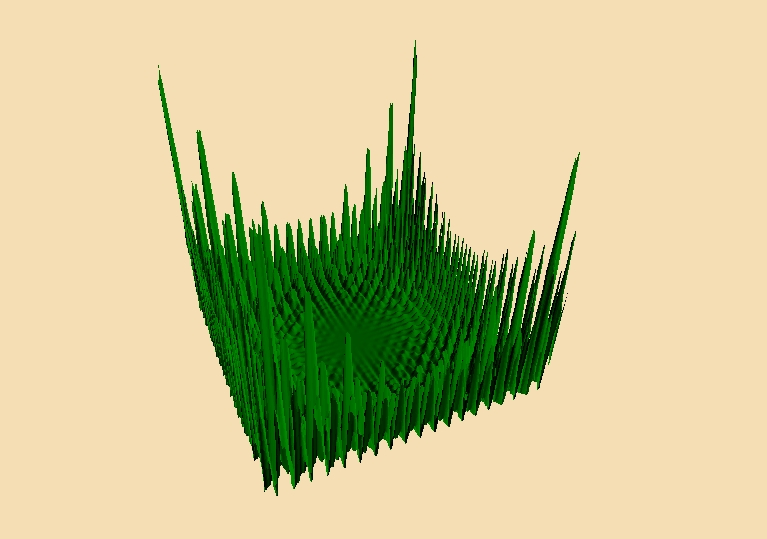
\includegraphics[scale=0.6]{/Users/guoyixuan/Documents/NTPU_STAT/images/Rplot64.jpeg}
    \caption{範例圖}
    \label{fig:scale}
  \end{figure}
\end{lstlisting}

\begin{figure}[H]
    \centering
        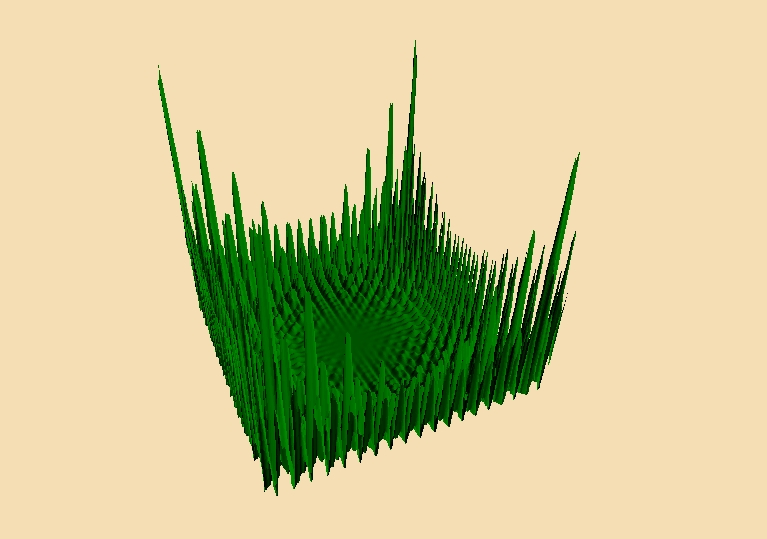
\includegraphics[scale=0.6]{/Users/guoyixuan/Documents/NTPU_STAT/images/Rplot64.jpeg}
    \caption{範例圖 (jpeg圖)}
    \label{fig:scale}
\end{figure}

圖形的大小可以透過一些指令來進行變化,我們可以利用 scale 來使原圖縮小,或者利用 width 將原圖縮小成內文行寬的 a 倍,其調整依等比例進行縮放。在圖 \ref{fig:scale} 中,本文件已經示範了在 \LaTeX 中插入 JPEG 圖,接著我們示範如何在文件中插入 EPS 檔案與 PNG 檔案,並使兩個檔案並排顯示。其中我們利用 {\A $\backslash$imgdir} 定義一個與編譯文章路徑相同的子目錄,如圖 \ref{fig:parallel}。

\textbf{圖片並排}

\bigskip
\begin{lstlisting}
   \begin{figure}[H]
    \centering
        \subfloat[範例圖 (eps圖)]{
        \includegraphics[scale=0.35]{\imgdir Rplot65.eps}}
        \subfloat[範例圖 (png圖)]{
        \includegraphics[scale=0.5]{\imgdir AnyConv.com__Rplot68.png}}
    \caption{圖形並排的作法}
    \label{fig:parallel}
  \end{figure}
\end{lstlisting}

\begin{figure}[H]
    \centering
        \subfloat[範例圖 (eps圖)]{
        \includegraphics[scale=0.35]{\imgdir Rplot65.eps}}
        \subfloat[範例圖 (png圖)]{
        \includegraphics[scale=0.5]{\imgdir AnyConv.com__Rplot68.png}}
    \caption{圖形並排的作法}
    \label{fig:parallel}
\end{figure}

\textbf{文字與圖片並排}\\
跟表格一樣,在 \LaTeX 中同樣可以使用 {\A $\backslash$minipage} 使文字與圖片並排呈現。

\begin{minipage}{.4\linewidth}
{\A minipage} 是另一種控制圖形位置的方式,適合必須與文字密切貼近的圖形。讓文字描述圖形時,可以用左圖或右圖,而不是依賴圖形編號。譬如,右圖示範的圖檔格為 PDF。此時,因為不能用 \verb|\begin{figure}|,沒有{\A label} 與  {\A caption}。

\end{minipage}
\begin{minipage}{.6\linewidth}
    \includegraphics[scale=0.6]{\imgdir Rplot62.jpeg}
\end{minipage}

\textbf{圖片旋轉}

\bigskip
\begin{lstlisting}
  \begin{figure}[H]
    \centering
        \includegraphics[angle=30,width=15cm, height=10cm]{\imgdir Rplot56.jpeg}
    \caption{旋轉圖片}
    \label{fig:angle}
  \end{figure}
\end{lstlisting}

\begin{figure}[H]
    \centering
        \includegraphics[angle=30,width=15cm, height=10cm]{\imgdir Rplot56.jpeg}
    \caption{旋轉圖片}
    \label{fig:angle}
\end{figure}

\end{document}






